\documentclass[12pt, twoside]{article}
\usepackage[letterpaper, margin=1in, headsep=0.5in]{geometry}
\usepackage[english]{babel}
\usepackage[utf8]{inputenc}
\usepackage{amsmath}
\usepackage{amsfonts}
\usepackage{amssymb}
\usepackage{tikz}
\usetikzlibrary{quotes, angles}
\usepackage{graphicx}
\usepackage{enumitem}
\usepackage{multicol}
\usepackage{hyperref}

\newif\ifmeta
\metatrue %print standards and topics tags

\title{IB Mathematics}
\author{Chris Huson}
\date{September 2021}

\usepackage{fancyhdr}
\pagestyle{fancy}
\fancyhf{}
\renewcommand{\headrulewidth}{0pt} % disable the underline of the header
\raggedbottom


\fancyhead[LE]{\thepage}
\fancyhead[RO]{\thepage \\ Name: \hspace{4cm} \,\\}
\fancyhead[LO]{BECA / IB Math 01-Linear functions\\* 27 October 2021}

\begin{document}

\subsubsection*{PreQuiz: I can model arithmetic sequences}
Arithmetic sequences\\[0.25cm]
Terms: $u_n=u_1 + d(n-1)$\\[0.25cm]
Sum: $\displaystyle S_n= \frac{n}{2}(u_1 + u_n)$\\[0.25cm]

\begin{enumerate}
\item Given the arithmetic sequence $2, 7, 12, 17, \dots$
  \begin{enumerate}[itemsep=1cm]
    \item Find the common difference $d$.
    \item Write down the next term, $u_5$.
    \item Find the fifteenth term.\vspace{1cm}
    \item Find the sum of the first fifteen terms.
  \end{enumerate} \vspace{2cm}

\item In an arithmetic sequence the first term is 11 and the fourth term is 26.
  \begin{enumerate}[itemsep=2cm]
    \item Find the common difference $d$.
    \item Find the tenth term, $u_{10}$.\vspace{1cm}
    \item Find the sum of the first ten terms.
  \end{enumerate} \vspace{3cm}

\newpage
\item The second term of an arithmetic sequence is 16 and the seventh term is 6.
  \begin{enumerate}[itemsep=3cm]
    \item Find the common difference $d$.
    \item Find the first term, $u_{1}$.
    \item Find the sum of the first seven terms.
  \end{enumerate} \vspace{2cm}

\item The rate on a credit card is $18\%$ per annum. Find the total amount due on a \$250 purchase after one month (principal and interest). \vspace{3cm}

\item Robert takes out a 5 month loan to purchase and repair a used car for resale. The principal amount is 20,000 euros and interest rate is $7.50\%$ per annum. Find the interest Robert pays.
\newpage

Equations of a straight line: $f(x)=mx+c$, $ax+by+d=0$, $(y-y_1)=m(x-x_1)$\\[0.25cm]
Gradient: $\displaystyle m=\frac{y_2-y_1}{x_2-x_1}$ \vspace{1cm}
  
\item Given the linear function $f(x)=-2x+4$. \hfill [4]
\begin{multicols}{2}
\begin{enumerate}
  \item Write down it's slope.\\ $m=$
  \vspace{0.25cm}
  \item Write down it's $y$-intercept.\\ $b=$
  \vspace{0.25cm}
  \item Draw the function $f$ on the grid.
  \vspace{1cm}
  \item Label the $x$-intercept with its coordinates as an ordered pair.
\end{enumerate} \vspace{.5cm}
  \begin{center} 
  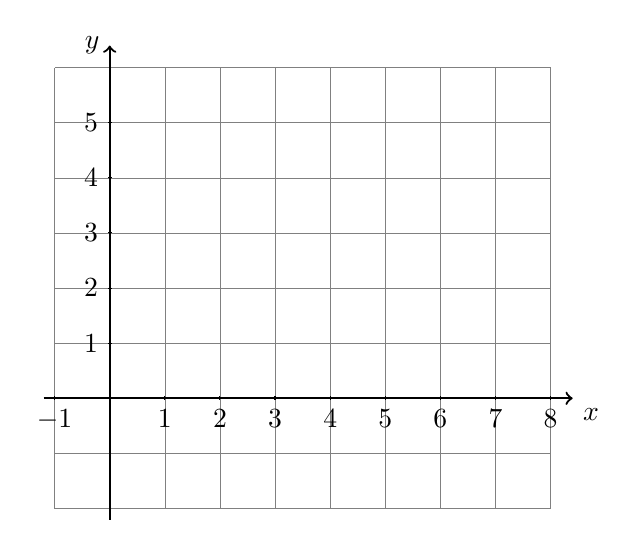
\begin{tikzpicture}[scale=0.7]
    \draw [help lines] (-1,-2) grid (8,6);
    \draw [thick, ->] (-1.2,0) -- (8.4,0) node [below right] {$x$};
    \draw [thick, ->] (0,-2.2)--(0,6.4) node [left] {$y$};
    \foreach \x in {-1,1,2,...,8} \draw (\x cm,1pt) -- (\x cm,-1pt) node[anchor=north] {$\x$};
    \foreach \y in {1, 2, 3, 4, 5} \draw (1pt,\y cm) -- (-1pt,\y cm) node[anchor=east] {$\y$};
    %\draw [thick, <->,smooth,samples=20,domain=-2.25:4.5] plot(\x,0.667*\x+2);
    %\fill (3,4) circle[radius=0.1] node[below right]{$Q$};
  \end{tikzpicture}
  \end{center}
\end{multicols}

\item The height of a plant $h$ in centimeters over a period of time $t$ measured in weeks is shown in the table. \hfill [3]
\begin{enumerate}
  \item Plot the data as points on the grid.
  \item Draw a line of best fit on the graph.
\end{enumerate}
  \begin{center} 
  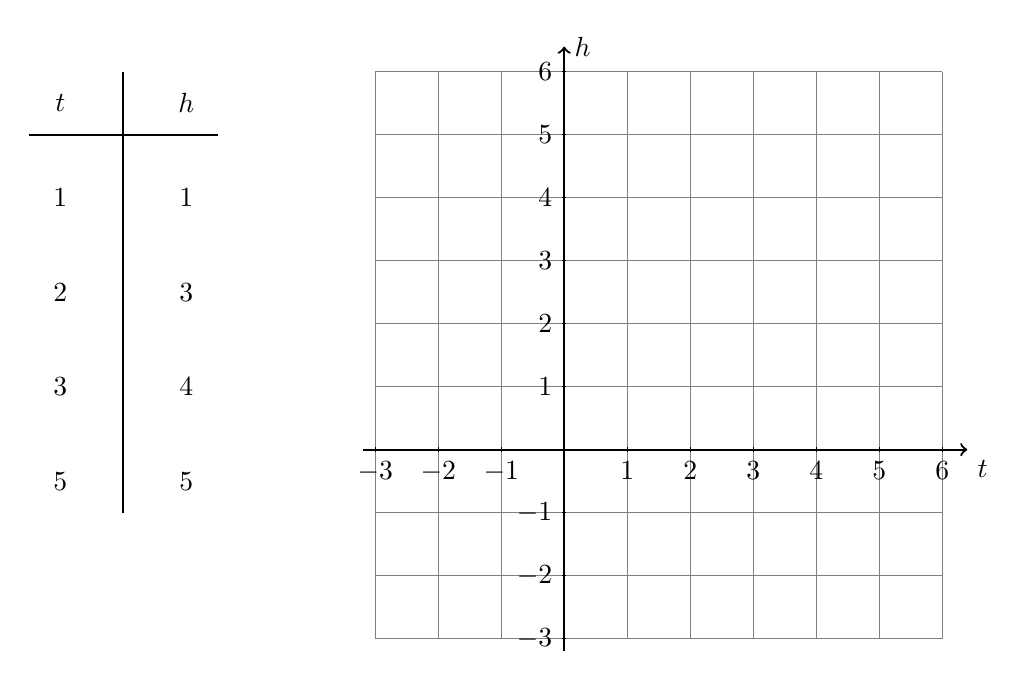
\begin{tikzpicture}[scale=0.8]
    \draw [help lines] (-3,-3) grid (6,6);
    \draw [thick, ->] (-3.2,0) -- (6.4,0) node [below right] {$t$};
    \draw [thick, ->] (0,-3.2)--(0,6.4) node [right] {$h$};
    \foreach \x in {-3,-2,-1,1,2,3,4,5,6} \draw (\x cm,1pt) -- (\x cm,-1pt) node[anchor=north] {$\x$};
    \foreach \y in {-3,-2,-1,1,2,3,4,5,6} \draw (1pt,\y cm) -- (-1pt,\y cm) node[anchor=east] {$\y$};

    \draw [thick] (-7,-1) -- (-7,6);
    \draw [thick] (-8.5,5) -- (-5.5,5);
    \node at (-8,5.5){$t$}; \node at (-6,5.5){$h$};

    \node at (-8,4){$1$}; \node at (-6,4){$1$};
    \node at (-8,2.5){$2$}; \node at (-6,2.5){$3$};
    \node at (-8,1){$3$}; \node at (-6,1){$4$};
    \node at (-8,-0.5){$5$}; \node at (-6,-0.5){$5$};
  \end{tikzpicture}
  \end{center}

\newpage
\item A function is defined over the domain $0 \leq x \leq 600$. Its intercepts are $(600,0)$ and $(0, 50)$. Draw the function on the grid. Number the $x$- and $y$-axes with an appropriate scale. \hfill [5]
  \begin{center}
  \begin{tikzpicture}[scale=1]
    %\draw [help lines] (-3,-2) grid (4,6);
    \draw [thick, ->] (-1.2,0) -- (10.4,0) node [below right] {$x$};
    \draw [thick, ->] (0,-1.2)--(0,10.5) node [right] {$y$};
    \foreach \x in {-1, 1,2, ..., 10} \draw (\x cm,4pt) -- (\x cm,-4pt);% node[anchor=north] {$\x$};
    \foreach \y in {1,2,..., 10} \draw (2pt,\y cm) -- (-2pt,\y cm);% node[anchor=east] {$\y$};
    %\fill (3,3) circle[radius=0.1] node[above right]{$(3,3)$};
    %\fill (6,-1) circle[radius=0.1] node[below left]{$(6,-1)$};
    %\draw [thick, <->,smooth,samples=20,domain=2.5:6.5] plot(\x,-1.33*\x+7);
  \end{tikzpicture}
  \end{center}

  \item Given $f(x)=\frac{3}{4}x+3$.  \hfill [2]
  \begin{enumerate}
    \item Find $f(8)$. \vspace{2cm}
    \item Find$f^{-1}(0)$.
  \end{enumerate} \vspace{4cm}

\newpage
\item The function $f(x)=-x^{2}+6x-6$ is shown on the graph. \hfill [8]
\begin{enumerate}
  \begin{multicols}{2}
      \item Write down its vertex as an ordered pair. \vspace{0.5cm}
      \item Draw on the graph the function \\$g(x)=-x+4$.
      \item Find the two ordered pairs that satisfy both $f$ and $g$. \vspace{3cm}
      \begin{center}
      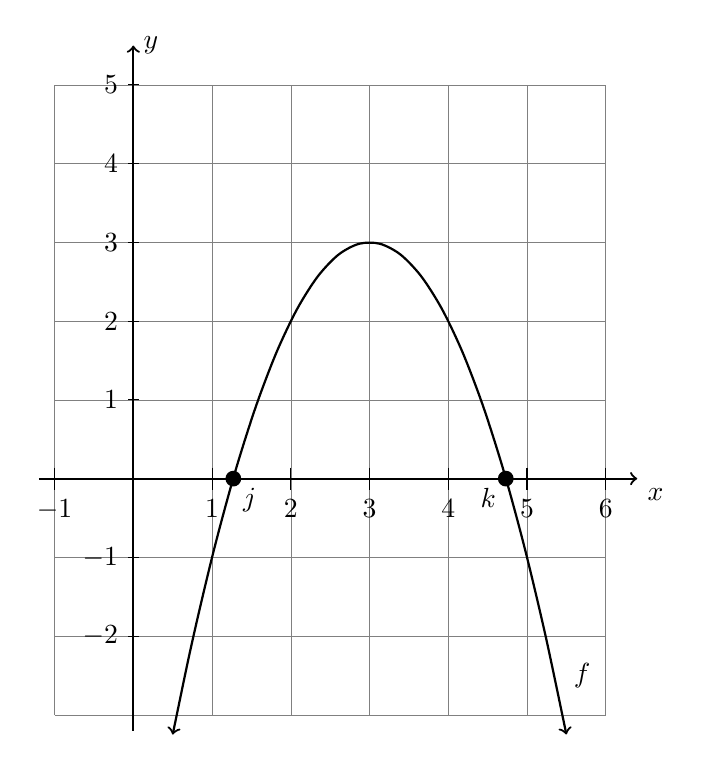
\begin{tikzpicture}[scale=1]
        \draw [help lines] (-1,-3) grid (6,5);
        \draw [thick, ->] (-1.2,0) -- (6.4,0) node [below right] {$x$};
        \draw [thick, ->] (0,-3.2)--(0,5.5) node [right] {$y$};
        \foreach \x in {-1, 1,2, ..., 6} \draw (\x cm,4pt) -- (\x cm,-4pt) node[anchor=north] {$\x$};
        \foreach \y in {-2,-1,1,2,..., 5} \draw (2pt,\y cm) -- (-2pt,\y cm) node[anchor=east] {$\y$};
        \fill (1.27,0) circle[radius=0.1] node[below right]{$j$};
        \fill (4.73,0) circle[radius=0.1] node[below left]{$k$};
        \draw [thick, <->,smooth,samples=20,domain=0.5:5.5] plot(\x,-\x*\x+6*\x-6);
        \node at (5.7,-2.5){$f$};
      \end{tikzpicture}
      \end{center}
    \end{multicols} 
    \vspace{2cm}
    \item Find the exact values of $j$ and $k$, the $x$-intercepts of $f$. (as an expression with radicals, not a decimal)
\end{enumerate} \vspace{3cm}


\end{enumerate}
\end{document}